% The "trap box" |x| + |y| <= M (a diamond) overlaid on the lattice of
% Z[sqrt(2)] under the canonical embedding: Minkowski's theorem will
% force a nonzero lattice point into the box.
% Source: book/tex/alg-NT/classgrp.tex (§ The trap box) — asy figure.
\documentclass[border=2mm]{standalone}
\usepackage{tikz}
\begin{document}
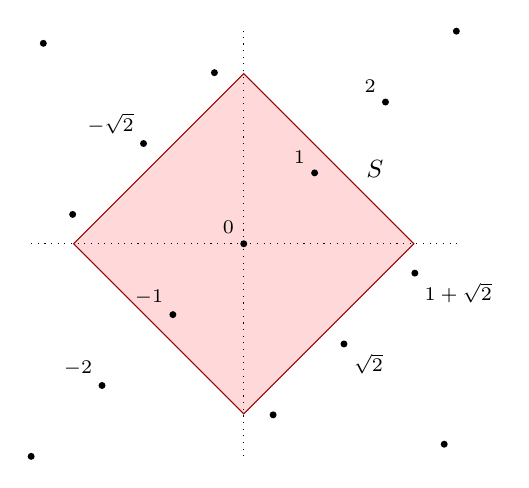
\begin{tikzpicture}[scale=0.9]
  \pgfmathsetmacro{\T}{sqrt(2)}
  \pgfmathsetmacro{\K}{2.4}
  \filldraw[fill=red!15, draw=red!60!black]
    (\K,0) -- (0,\K) -- (-\K,0) -- (0,-\K) -- cycle;
  \node[font=\small] at (2*\K/3+0.25,\K/3+0.25) {$S$};
  \draw[dotted] (-3,0) -- (3,0);
  \draw[dotted] (0,-3) -- (0,3);
  \foreach \a in {-10,...,10}
    \foreach \b in {-10,...,10}
    {
      \pgfmathsetmacro{\px}{\a+\T*\b}
      \pgfmathsetmacro{\py}{\a-\T*\b}
      \pgfmathparse{abs(\px)<=3 && abs(\py)<=3 ? 1 : 0}
      \ifnum\pgfmathresult=1
        \fill (\px,\py) circle (1.4pt);
      \fi
    }
  \node[above left, font=\scriptsize] at (-2,-2) {$-2$};
  \node[above left, font=\scriptsize] at (-1,-1) {$-1$};
  \node[above left, font=\scriptsize] at (0,0) {$0$};
  \node[above left, font=\scriptsize] at (1,1) {$1$};
  \node[above left, font=\scriptsize] at (2,2) {$2$};
  \node[above left, font=\scriptsize] at (-\T,\T) {$-\sqrt 2$};
  \node[below right, font=\scriptsize] at (\T,-\T) {$\sqrt 2$};
  \node[below right, font=\scriptsize] at (1+\T,1-\T) {$1+\sqrt 2$};
\end{tikzpicture}
\end{document}
